\section{System Explanation}
\label{ch2:sec:system-explanation}

\begin{figure}[htb]\centering
% Define some block styles
\tikzstyle{box} = [%
	draw,%
	rectangle,%
	%fill=green!20,%
	minimum height=3em,%
	minimum width=5em,%
]
\subfloat[]{%
	\begin{tikzpicture}[node distance=1.5cm, shorten >= 1pt, >=stealth', auto, scale=0.8, transform shape]
		% Define nodes
	    \path (0,0)
	    node [box, fill=blue!20](data) {Data}
	    node [box, fill=blue!20, below of=data](forecast) {Forecast}
	    node [box, fill=blue!20, below of=forecast](schedule) {Schedule}
	    node [box, below of=schedule](battery) {Battery}
	    node [box, below of=battery](network) {Network};
		% Draw lines
		\draw [->] (data) to (forecast);
		\draw [->] (forecast) to (schedule);
		\draw [->] (schedule) to (battery);
		\draw [->] (battery) to (network);
	\end{tikzpicture}%
	\label{ch2:subfig:traditional-forecast-based-system}%
}
\hspace{10mm}
\subfloat[]{
	\begin{tikzpicture}[node distance=1.5cm, shorten >= 1pt, >=stealth', auto, scale=0.8, transform shape]
		% Define nodes
	    \path
	    (0,0) 
	   	node [box, fill=green!20, below of=schedule, xshift=-14.5mm](controller) {Controller}
		node [box, fill=green!20, below of=controller](mpc) {MCP}
	    node [box, right of=controller, xshift=15mm](battery) {Battery}
	    node [box, below of=battery](network) {Network};;
		% Draw lines
		\draw [->] (network) to (mpc);
		\draw [->] (mpc) to (controller);
		\draw [->] (controller) to (battery);
		\draw [->] (battery) to (network);
	\end{tikzpicture}%
	\label{ch2:subfig:traditional-on-line-system}%
}
\hspace{10mm}
\subfloat[]{%
	\begin{tikzpicture}[node distance=1.5cm, shorten >= 1pt, >=stealth', auto, scale=0.8, transform shape]
		% Define nodes
	    \path
	    (0,0)
	    node [box, fill=blue!20](data) {Data}
	    node [box, fill=blue!20, below of=data](forecast) {Forecast}
	    node [box, fill=blue!20, below of=forecast](schedule) {Schedule}
	    node [box, below of=schedule](battery) {Battery}
	    node [box, below of=battery](network) {Network}
	   	node [box, fill=green!20, left of=battery, xshift=-14.5mm](controller) {Controller}
		node [box, fill=green!20, below of=controller](mpc) {MCP};
		% Draw lines
		\draw [->] (data) to (forecast);
		\draw [->] (forecast) to (schedule);
		\draw [->, bend right] (schedule.180) to (controller.90);
		\draw [->] (network) to (mpc);
		\draw [->] (mpc) to (controller);
		\draw [->] (controller) to (battery);
		\draw [->] (battery) to (network);
	\end{tikzpicture}%
	\label{ch2:subfig:proposed-hybrid-system}%
}

\caption{Combination of traditional forecast driven BESS control (Subfig. \ref{ch2:subfig:traditional-forecast-based-system}) and traditional on-line system (Subfig. \ref{ch2:subfig:traditional-on-line-system}) results in the proposed hybrid system (Subfig. \ref{ch2:subfig:proposed-hybrid-system}).}
\label{ch2:fig:system-diagram}
\end{figure}


The underlying research project was conducted in collaboration with the \textit{Energy Networks} division of the British DNO \textit{Scottish and Southern Energy} (SSE-EN) \cite{NTVV2016}.
For their field trial, they developed a forecast driven and an on-line control method to control their street-level connected BESS.
The diagram in Figure \ref{ch2:fig:system-diagram} shows these two control methods and their main system constituents, alongside the proposed hybrid system.
Here, the two underlying traditional systems in Figure \ref{ch2:subfig:traditional-forecast-based-system} and \ref{ch2:subfig:traditional-on-line-system}, encapsulate off-line and on-line BESS control, respectively.
Entailing the benefits from both the traditional forecast driven and the on-line BESS control, the proposed dynamic control (in Figure \ref{ch2:subfig:proposed-hybrid-system}) is therefore titled the hybrid system.

Battery and network model are common constituents amongst all three systems.
Therefore, the battery model that is used in this work is explained first.
Afterwards, the data acquisition, forecasting and BESS scheduling is explained, since scheduling is performed whilst with battery constraints.
The next section then entails the dynamic control, i.e. the two green constituent system blocks that control BESS operation.

\subsection{BESS model}

The model of the system has been defined to coincide with the physical device that was deployed by SSE-EN.
Therefore, the model had to accurately capture the physical limitations of the device, which include a limited capacity of the battery pack, $C_{battery}$, and a corresponding charge and discharge factor (i.e. the ``C-factor''), $C_{factor}$.
Self-discharge losses inside the battery pack were captured as the ratio $\eta$, where $\eta \in (0, 1)$ and represented the energy that was lost over time due to the battery's imperfect means of storing charge.
Units containing power electronics to regulate the three-phase power flow into and out of the BESS also had power ratings, $P_{rating}$, which must not be exceeded.
Correspondingly, conversion loss leading into a BESS round-trip efficiency, $\mu$, where $\mu \in (0, 1)$, was also included in the model.

Since the model was simulated, a finite time between each simulation step had to be defined, $\tau$.
Therefore, the change in SOC, i.e. $\delta SOC(t)$, can be computed as the difference in the current SOC, $SOC(t)$, and the next SOC, $SOC(t+\tau)$.
Combining this with the self-discharge loss, the following SOC equation is defined:

\begin{equation}
	SOC(t+\Delta t) := \eta(SOC(t) + \delta SOC(t))
	\label{ch2:equ:soc-equation}
\end{equation}

However, this change in SOC is the result of charging or discharging the battery by injecting or releasing energy.
The amount of energy that flows into or out of the BESS is defined by the active power that is consumed, $p(t)$.
Here, the sign of the BESS power indicates whether the device is charging or discharging.
To behave similar to a load in a network, positive power was associated to charging and therefore negative power represented discharging the BESS.
The amount of actual charge stored in the battery differs from the due to the aforementioned conversion efficiency, $\eta$.
In order to deliver the correct BESS power, a conversion to the system's battery power was defined:

\begin{equation}
	p_\text{bat}(t) =
	\begin{cases}
		\mu p(t) &\text{if } p(t) \geq 0\\
		\frac{1}{\mu}p(t) &\text{otherwise}
	\end{cases}
	\forall t
	\label{ch2:equ:battery-power}
\end{equation}

Therefore, the amount of energy injected into the battery during $\tau$ can also be determined based upon the battery power, i.e.:

\begin{equation}
	\delta SOC(t) = \frac{\tau}{C_{battery}}p_{battery}(t)
	\label{ch2:equ:soc-equation-from-battery-power}
\end{equation}

Combining Equation \ref{ch2:equ:soc-equation} and \ref{ch2:equ:soc-equation-from-battery-power} and solving for $SOC(t+\tau)$, yields the following battery model equation:

\begin{equation}
	SOC(t+\tau) =
	\begin{cases}
		\mu \left(SOC(t) + \eta \frac{\tau}{C_{battery}}p(t)\right) &\text{if } p(t) \geq 0\\
		\mu \left(SOC(t) + \frac{1}{\eta} \frac{\tau}{C_{battery}}p(t)\right) &\text{otherwise}
	\end{cases}
	\forall t
	\label{ch2:equ:battery-model-equation}
\end{equation}

For the purpose of the simulation, it is assumed that the battery is initially charged up to 50\%.
Hence, the initial conditions of this model are defined as $SOC(0) = 0.5$, which makes the model valid for a time span of $t \geq 0$.

\subsection{Load data and BESS scheduling}

Having established the BESS model, the procedure to generate a corresponding schedule is explained.
Following common scheduling practice and for the reasons mentioned in the literature review, this schedule was generated at half-hourly resolution.
Since BESS operation is performed at a sub-half-hourly period, i.e. $\tau$, the schedule's period is denoted as $\kappa$.
It is worth mentioning, that the scheduled BESS power is assumed constant over the scheduling period $\kappa$.
With this assumption and the knowledge of the BESS's SOC, it is possible to interpolate the change in SOC during $\kappa$.
This feature is used to link the sub-half-hourly BESS operation to its half-hourly power schedule.

In order to generate the schedule a load forecast, $p_{forecast}(k)$, was required.
This forecast, similar to the schedule, is also at half-hourly resolution and was provided by SSE-EN as part of the research project.
The task at hand was to find a half-hourly BESS schedule, $p_{schedule}(k)$, that improves the shape of the underlying forecast.
In order to generate an optimised BESS schedule, a mechanism to quantify improvements had to be defined before the problem to solve for $p_{schedule}(k)$ can be formalised.
Three cost-functions are used that capture these improvements when minimised.

These costs entailed the Peak-to-Average Ratio (PAR), the difference between the resulting power profile's maximum and minimum load, and the magnitude of all power transients \cite{Mohsenian-Rad2010, Mostafa2016}.
The first cost function, which addresses the minimisation of PAR is defined as follows:

\begin{equation}
	\zeta_{PAR}(\textbf{p}) := \frac{\max_t|\textbf{p}|}{\overline{\textbf{p}}} - 1%\frac{\max_t|p(k(t))|}{\frac{1}{T}\sum_{t=1}^Tp(k(t))} - 1
	\label{ch2:equ:cost-par}
\end{equation}

Here, $K$ is the length of the scheduling horizon, which is equal to the forecast length, too.
A perfect power profile that yields a PAR of zero would be a perfectly flat power profile.
However, due to limited battery capacity, achieving such a cost is highly unlikely.
The second cost function represents the difference between minimum and maximum power:

\begin{equation}
	\zeta_\text{MMD}(\textbf{p}) := (\max_t(\textbf{p}) - \min_t(\textbf{p}))^2
	\label{ch2:equ:cost-min-max}
\end{equation}

Similar to the PAR, this cost also reduces to zero when the resulting power profile is a perfectly flat line.
Unlike the PAR, this cost is insensitive to mean power adjustments.
Therefore, unnecessary and potentially damaging battery cycling in order to elevate the profile's mean is avoided when this cost is included alongside PAR.
So far, $\zeta_{PAR}$ and $\zeta_{MM}$ only impact the fringes of the resulting half-hourly power profile.
The final cost therefore addresses the interim power volatility by aiming to minimise the largest possible power transient:

\begin{equation}
	\zeta_\text{TRA}(\textbf{p}) := \max_{t}(p(t+\Delta t)-p(t))^2
	\label{ch2:equ:cost-tra}
\end{equation}

Minimising this final cost therefore has a smoothening effect on the improved half-hourly power profile.
All three cost functions are summaries into a single global cost function, where only the half-hourly BESS schedule is seen as an input and the forecast is kept as constant:

\begin{equation}
\begin{split}
	\zeta(\textbf{p}_{sch}) := &\zeta_\text{PAR}(\textbf{p}_{sch}+	\textbf{p}_{for})\\
	&+ \zeta_\text{MM}(\textbf{p}_{sch}+\textbf{p}_{for})\\
	&+ \zeta_\text{TRA}(\textbf{p}_{sch}+\textbf{p}_{for})
\end{split}
\label{ch2:equ:cost-global}
\end{equation}

Subject to BESS constraints, this global cost function was then minimised using Sequential Quadratic Programming (SQP) to yield a BESS schedule that is optimised for the given forecast:

\begin{equation}
	\min_{\textbf{p}_{sch}}\zeta(\textbf{p}_{sch})
	\text{ s.t. }
	\begin{cases}
		SOC_{tol} \leq SOC(t)\\
		SOC(t) \leq 1-SOC_{tol}\\
		|p_{bat}(t)| \leq C_{bat} \times C_{f}
	\end{cases}
\label{ch2:equ:cost-minimisation}
\end{equation}

To visualise this schedule optimisation, a three day sample schedule was generated using the cost minimisation as it is defined in Eq. \ref{ch2:equ:cost-minimisation}.
To generate this sample BESS schedule, three forecasted days were separately evaluated and a half-hourly BESS schedule was generated for each day.
Then, the actual sub-half-hourly demand was used and the half-hourly BESS schedule was applied to emphasise the disparity in peak load magnitude and timing.

\begin{figure}\centering
	\subfloat[]{%
		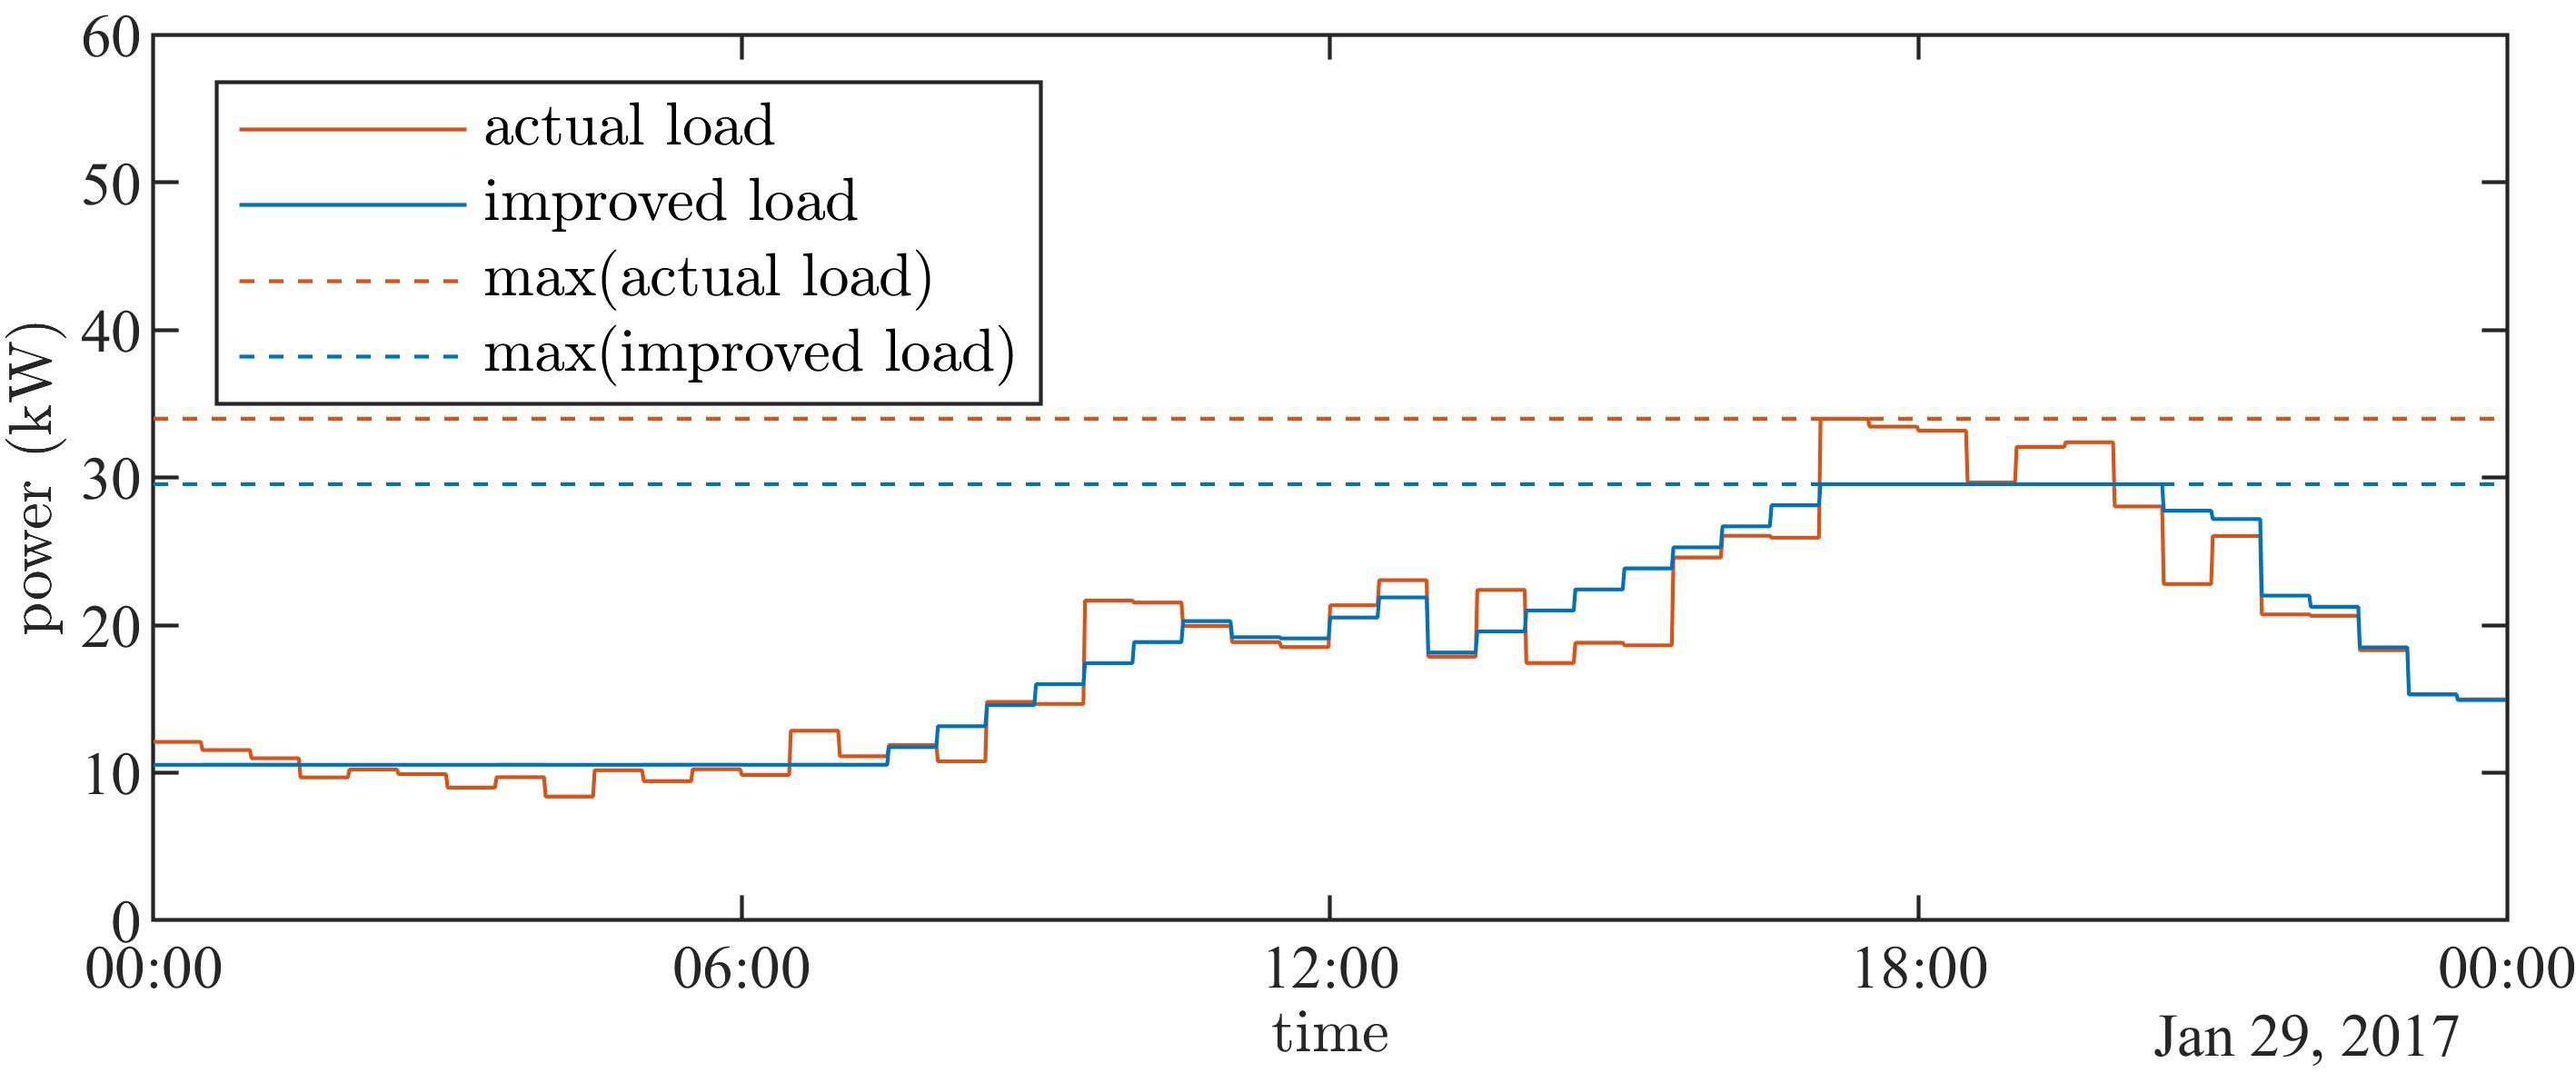
\includegraphics{_chapter2/fig/day-forecasted}
		\label{ch2:subfig:day-forecasted}
	}\\
	\subfloat[]{%
		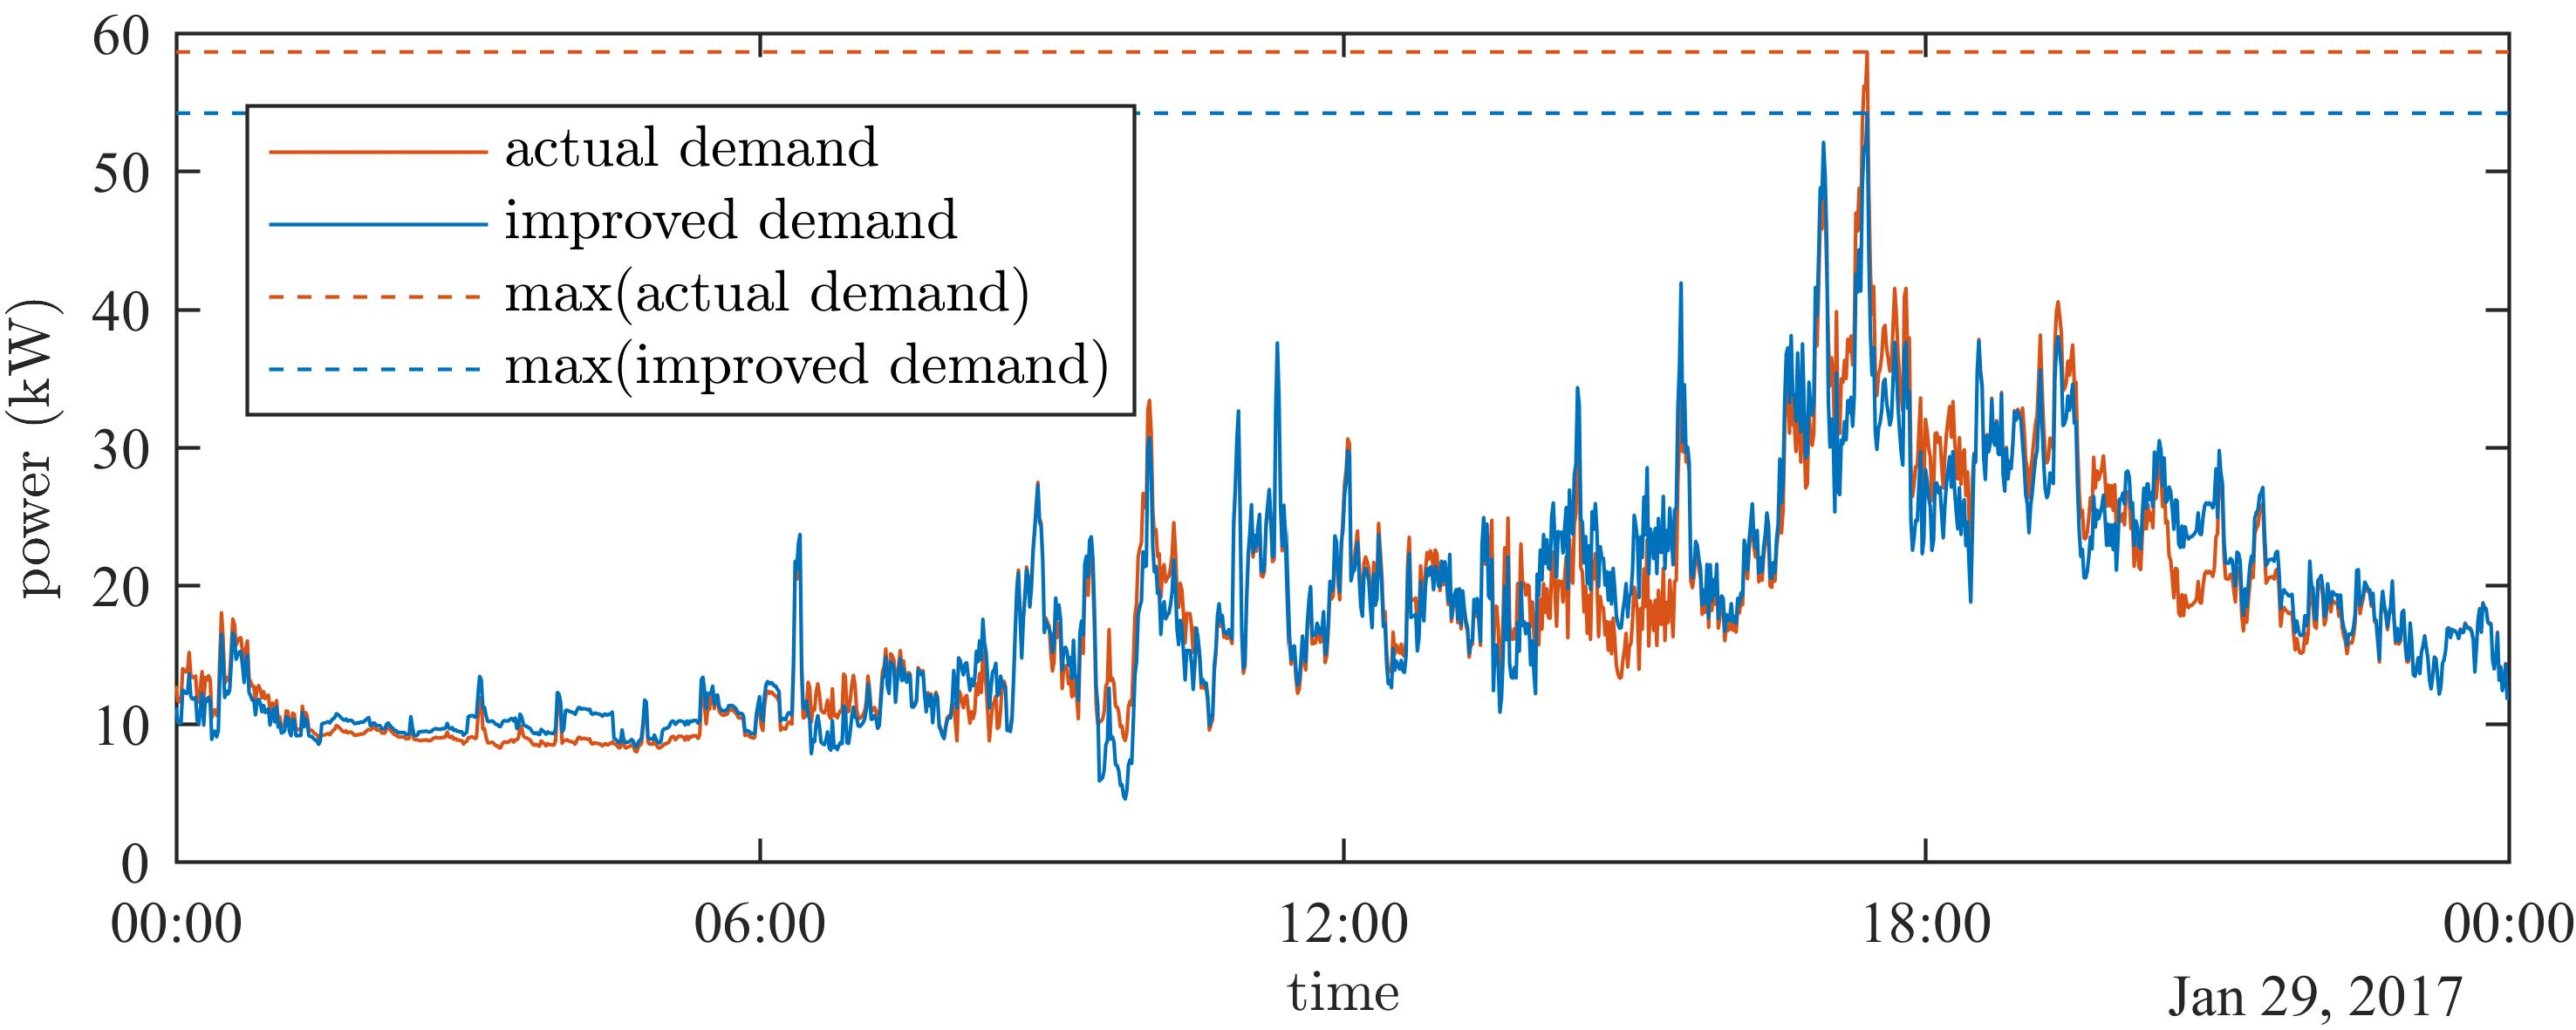
\includegraphics{_chapter2/fig/day-actual}
		\label{ch2:subfig:actual-forecasted}
	}
	\caption{An example of applying a half-hourly ESMU schedule to the half-hourly substation load (Subfig. \ref{ch2:subfig:day-forecasted}) and the actual, sub-half-hourly daily load, measured at the substation (Subfig. \ref{ch2:subfig:actual-forecasted}).}
	\label{ch2:fig:cost-sample}
\end{figure}

This example in Figure \ref{ch2:fig:cost-sample} highlights the potential incompatibility between half-hourly BESS schedules and the actual sub-half-hourly load.
As previously discussed, benefits of BESS were intended to mitigate high resolution volatility, yet this cannot be achieved when applying BESS schedules in an open-loop manner.
Therefore, in the next section, the control strategy to add an on-line component is explained.




 